%\documentclass[11pt,a4paper]{scrartcl}
\documentclass{MSM_latex}
\author{M. Denkinger, S. Eyselein, J. Schnitzler}


\makeatletter
\let\runauthor\@author
\let\rundate\@date
% Fußzeile
\lfoot{\textit{\runauthor} \\ \textit{\rundate}}
%%%%%%%%%%%%%%%%%%%%%%%%%%%%%%%%%%%%%%%%%%%%%%%%%%%5
% Matlab-Code
\usepackage{listings}
\usepackage{color}

\definecolor{mygreen}{rgb}{0,0.6,0}
\definecolor{mygray}{rgb}{0.5,0.5,0.5}
\definecolor{mymauve}{rgb}{0.58,0,0.82}

\lstset{ %
  backgroundcolor=\color{white},   % choose the background color
  basicstyle=\footnotesize,        % size of fonts used for the code
  breaklines=true,                 % automatic line breaking only at whitespace
  captionpos=b,                    % sets the caption-position to bottom
  commentstyle=\color{mygreen},    % comment style
  escapeinside={\%*}{*)},          % if you want to add LaTeX within your code
  keywordstyle=\color{blue},       % keyword style
  stringstyle=\color{mymauve},     % string literal style
  language=Matlab,                 % the language of the code
  numbers=left,                    % where to put the line-numbers; possible values are (none, left, right)
  numbersep=5pt,                   % how far the line-numbers are from the code
  numberstyle=\tiny\color{mygray}, % line-number style
  rulecolor=\color{black},         % if not set, the frame-color may be changed on line-breaks within not-black text
  showspaces=false,                % show spaces everywhere adding particular underscores; it overrides 'showstringspaces'
  showstringspaces=false,          % underline spaces within string literals
  showtabs=false,                  % show tabs within string literals adding particular underscores
  stepnumber=2,                    % the step between two line-numbers. If it's 1, each line will be numbered
  tabsize=2,                       % sets default tabsize to 2 spaces
  title=\lstname                   % show the filename of files included with \lstinputlisting; also try caption instead of title
}


\begin{document}


\section{Weihnachtsprojekt: Simulation und Regelung eines Knickarmroboters}

\subsection*{Aufgabe 1 - Bestimmung der Kinematik und DH-Parameter}

Zur Bestimmung der Kinematik ist es notwendig herauszufinden, wie die einzelnen Gelenke des Roboters miteinander verbunden sind.
Die Denavit-Hartenberg-Notation wird verwendet, um die 3D-Transformation zum nächsten Gelenk mithilfe von vier Parameter zu beschreiben. Im Fall des Knickarmroboters ist
dies sehr einfach, da es sich lediglich um eine Kette von drei Gelenken handelt. Die Koordinatentransformation ist jeweils eine Rotation um die $z$-Achse mit $\theta_i$
und eine Translation in der $xy$-Ebene, um die Länge $a_i = l_i$. Wir können somit das erste Gelenk in den Ursprung legen und mithilfe von zwei Transformationen $T_{12}$ und $T_{23}$ alles beschreiben. Um mit einem nicht gedrehten Koordinatensystem anzufangen, benötigen wir zusätzlich $T_{01}$. Die DH-Parameter sind in Tabelle \ref{tab:DH} aufgeführt.



\begin{table}[tb]
	\centering
	\begin{tabular}{lccccr}
		\toprule
		Achse & $a_{i-1}$ & $\alpha_{i-1}$ & $d_i$ & $\theta_i$ & Art \\
		\midrule
		1 & 0& 0& 0& $-90^\circ $& Rotation \\
		2 & $l_1 = 0.16 \text{ m}$& 0& 0& $\alpha$& Translation\\
		3 & $l_2 = 0.128 \text{ m}$& 0& 0& $\beta$& Both\\ 
		\bottomrule
	\end{tabular}
	\caption{DH-Parameter des Knickarmroboters}
	\label{tab:DH}
\end{table}

Daraus resultieren die Transformationsmatrizen
\begin{equation*}
	T_{12}(\alpha, l_1) = \begin{pmatrix}
	\cos(\alpha) & -\sin(\alpha) & 0 & 0 \\
	\sin(\alpha) & \cos(\alpha) & 0 & 0 \\
	0 & 0 & 1 & 0 \\
	0 & 0 & 0 & 1
	\end{pmatrix} \cdot \begin{pmatrix}
	1 & 0 & 0 & l_1 \\
	0 & 1 & 0 & 0 \\
	0 & 0 & 1 & 0 \\
	0 & 0 & 0 & 1
	\end{pmatrix} = \begin{pmatrix}
	\cos(\alpha) & -\sin(\alpha) & 0 & \cos(\alpha) l_1 \\
	\sin(\alpha) & \cos(\alpha) & 0 & \sin(\alpha) l_1 \\
	0 & 0 & 1 & 0 \\
	0 & 0 & 0 & 1
	\end{pmatrix}
\end{equation*}
und
\begin{equation*}
	T_{23}(\beta, l_2) = \begin{pmatrix}
	\cos(\beta) & -\sin(\beta) & 0 & 0 \\
	\sin(\beta) & \cos(\beta) & 0 & 0 \\
	0 & 0 & 1 & 0 \\
	0 & 0 & 0 & 1
	\end{pmatrix} \cdot \begin{pmatrix}
	1 & 0 & 0 & l_2 \\
	0 & 1 & 0 & 0 \\
	0 & 0 & 1 & 0 \\
	0 & 0 & 0 & 1
	\end{pmatrix} = \begin{pmatrix}
	\cos(\beta) & -\sin(\beta) & 0 & \cos(\beta) l_2 \\
	\sin(\beta) & \cos(\beta) & 0 & \sin(\beta) l_2 \\
	0 & 0 & 1 & 0 \\
	0 & 0 & 0 & 1
	\end{pmatrix}
\end{equation*}

Die Gesamttransformation ergibt sich aus der Multiplikation der beiden Matrizen, welche mithilfe von trigonometrischen Additionstheoremen vereinfacht werden kann.

\begin{equation*}
	T_{13} = T_{12} \cdot T_{23} = \begin{pmatrix}
	\cos(\alpha + \beta) & -\sin(\alpha + \beta) & 0 & \cos(\alpha) l_1 + \cos(\alpha + \beta) l_2\\
	\sin(\alpha + \beta) & \cos(\alpha + \beta) & 0 & \sin(\alpha) l_1 + \sin(\alpha + \beta) l_2 \\
	0 & 0 & 1 & 0 \\
	0 & 0 & 0 & 1
	\end{pmatrix}
\end{equation*}

\begin{equation*}
	T_{03} = \begin{pmatrix}
	\cos(\alpha + \beta) & -\sin(\alpha + \beta) & 0 & \cos(\alpha) l_1 + \cos(\alpha + \beta) l_2\\
	\sin(\alpha + \beta) & \cos(\alpha + \beta) & 0 & \sin(\alpha) l_1 + \sin(\alpha + \beta) l_2 \\
	0 & 0 & 1 & 0 \\
	0 & 0 & 0 & 1
	\end{pmatrix}
\end{equation*}

Somit ergibt sich die Position von Gelenk 2 im Weltkoordinatensystem zu
\begin{equation*}
	\begin{pmatrix} x_2 \\ y_2 \\ z_2 \end{pmatrix} = \begin{pmatrix}
	\cos(\alpha) l_1\\ \sin(\alpha) l_1 \\ z_2 \end{pmatrix}
\end{equation*}
und die Position von Gelenk 3 bzw. des Endeffektors zu
\begin{equation*}
	\begin{pmatrix} x_3 \\ y_3 \\ z_3 \end{pmatrix} = 
	\begin{pmatrix}
	\cos(\alpha) l_1 + \cos(\alpha + \beta) l_2\\ \sin(\alpha) l_1 + \sin(\alpha + \beta) l_2 \\ z_3 
	\end{pmatrix}
\end{equation*}

\textit{Anmerkung}: Da die Parameter $\alpha_{i-1}$ und $d_i$ sind immer null sind, ist eine 2D Betrachtung ausreichend, wie man auch an der \emph{Identitäts-Zeile-Spalte} für $z$ erkennen kann.
\subsection*{Aufgabe 2 - Bestimmung der Bewegungsgleichung}

\subsubsection*{Generalisierte Koordinaten}
Die Wahl fällt zu $y(1) = \alpha$ und $y(2) = \beta$. 
Die generalisierten Koordinaten sind somit die Winkel der Gelenke 1 und 2.

\subsubsection*{Lagrang'sche Gleichung 2. Art}
Die Bewegungsgleichung des Arms kann mit folgender Gleichung beschrieben werden:

\begin{equation}
	M(y) \cdot \ddot{y} + D(y,\dot{y}) \cdot \dot{y} + g(y) = \tau_{Reib} + \tau_{Aktormoment}
\end{equation}

Dabei berechnet sich die Massenmatrix $M_{i}$ mit $M = \sum_{i}{M_{i}}$ von Arm i nach:
\begin{equation}
	M_{i}(y) = \left[m_{i}J_{TiS}^{T}(y) \cdot J_{TiS}(y) + 
	J_{RiS}^{T}(y) \cdot S_{0,iS}(y) \cdot I_{iS,iS} \cdot S_{0,is}^{T}(y) J_{RiS}(y) \right]
\end{equation}

Dabei sind $J_{TiS}(y)$ und $J_{RiS}(y)$ die Jakobimatrizen für den Schwerpunkt für Körper 
i der Translation beziehungsweise Rotation und $I_{iS,iS}$
der Trägheitstensor von Körper i dargestellt in dessen Schwerpunkt.

Mithilfe der Transformationsmatrix $S_{0,iS}(y)$ kann der Trägheitstensor im Inertialsystem dargestellt werden:
\begin{equation}
	I_{iS,0} = S_{0,iS}(y) \cdot I_{iS,iS} \cdot S_{0,is}^{T}(y)
\end{equation}


Für  $D(y,\dot{y})$ gilt:
\begin{equation}
	D_{kj} = \sum_{i=1}^{n}h_{ijk}(y)\dot{y}_{i}
\end{equation}
mit den Christoffel-Symbolen
\begin{equation}
	h_{ijk} = \frac{1}{2}\left(	\frac{\partial M_{kj}}{\partial y_{i}} + 
								\frac{\partial M_{ki}}{\partial y_{j }} -
								\frac{\partial M_{ij}}{\partial y_{k}}				\right)
\end{equation}

Der Graviationsvektor $g(y)$ ist definiert als
\begin{equation}
	g(y) = \left[ 
			\frac{\partial{V}}{\partial{y_{1}}} , 
			\frac{\partial{V}}{\partial{y_{2}}}
	\right]^{T}
\end{equation}

mit der potentiellen Energie $V$:
\begin{equation}
	V(y) = \sum_{i}V_{i} = \sum_{i}m_{i}g \cdot p_{iS,0}(y) 
\end{equation}
nach 2.1.11 Lagrange'sche Gleichungen zweiter Art in \cite{Fehr23}.
Die Umsetzung der genannten Gleichungen wurde mit der Symbolic Math Toolbox in Matlab implementiert.
Gleichung (1) liefert dann jeweils eine Differentialgeichung pro generalisierte Koordinate $y_{i}$.



\subsubsection*{Reibungsterm}
In Gleichung (1) geht das Reibmoment der Lagerung der Arme $\tau_{Reib}$ mit ein, welches aus der Überlagerung der viskosen mit der 
statischen Reibung modelliert wird:

\begin{figure}[H]
	\centering
	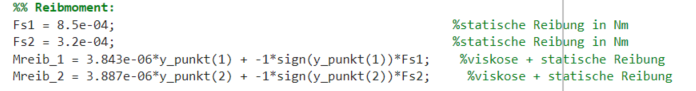
\includegraphics[width=0.95\textwidth]{Reibung.png}
	\caption{Modellierung der Lagerreibung}
\end{figure}

\subsection*{Aufgabe 3 - Trajektorienplanung}


Die vorliegende Trajektorienplanung beschäftigt sich mit der Definition und Berechnung von Trajektorien für einen Robotermanipulator. Das Ziel der Trajektorie wird dabei in globalen Koordinaten angegeben und ist durch den Vektor \( y_{\text{end\_glob}} \) definiert. Dieser Vektor repräsentiert die gewünschte Endposition des Endeffektors des Roboters.

\begin{verbatim}
    Ziel in globalen Koordinaten
    y_end_glob = [4*sqrt(6)-4*sqrt(2)-10; ...
                 -4*sqrt(6)-4*sqrt(2)-10*sqrt(3); 0]/125;
\end{verbatim}

Um die Trajektorie zu planen, müssen zuerst die globalen Koordinaten in Gelenkwinkel umgerechnet werden. Aus der Kinematik ergibt sich folgende Funktion zum Bestimmen der Gelenkwinkel. Dabei ist \(q(1)\) der Winkel \(\alpha\) und \(q(2)\) der Winkel \(\beta\). Die Funktion \texttt{pos\_endeff} gibt die Endposition in globalen Koordinaten abhängig von den Gelenkwinkeln \(\alpha\) und \(\beta\) an.  Weiterhin berechnet die Funktion \texttt{to\_endeff} den Abstand zwischen der Endeffektorposition und der Startposition, abhängig von den Gelenkwinkeln. Sobald \texttt{to\_endeff} Null ist, befindet sich der Endeffektor an der gewünschten Position. Die Funktion \texttt{q\_end} löst dies mit den Anfangsbedingungen \(q_0\) und gibt die Gelenkwinkel für die Endposition zurück.

\begin{verbatim}
    pos_endeff = @(q) 4/25*[sin(q(1)) + 4/5*sin(q(1)+q(2)); ...
    - cos(q(1)) - 4/5*cos(q(1)+q(2)); 0];
    to_endeff = @(q) pos_endeff(q) - y_end_glob;
    q_0 = [y_0(1); y_0(3)];
    q_end = fsolve(to_endeff, q_0);
\end{verbatim}

Mit den berechneten Winkeln kann die Trajektorienplanung beginnen. Wir haben uns für einen quintic spline entschieden, da dort sowohl Lage, Geschwindigkeit und Beschleunigung der Start- und Endlage vorgegeben werden können.
 Es müssen die Koeffizienten der Polynome 5.ten Grades berechnet werden.

 \begin{verbatim}
    a_poly = @(t)  a_coef(1) + a_coef(2)*(t-t_0) + a_coef(3)*(t-t_0).^2 
                 + a_coef(4)*(t-t_0).^3 + a_coef(5)*(t-t_0).^4 + a_coef(6)*(t-t_0).^5;
   
    b_poly = @(t)  b_coef(1) + b_coef(2)*(t-t_0) + b_coef(3)*(t-t_0).^2
                 + b_coef(4)*(t-t_0).^3 + b_coef(5)*(t-t_0).^4 + b_coef(6)*(t-t_0).^5;
\end{verbatim}

Die Anfangs- und Endbedingungen werden in \texttt{a\_init} und \texttt{b\_init} definiert. Dabei sind die Lage, die Geschwindigkeit und die Beschleunigung für Anfangs- und Endlage beschrieben.

\begin{verbatim}
    t_0 = tspan(1);
    t_end = tspan(2);
    a_init = [ q_0(1); y_0(2); 0;  q_end(1); 0; 0];
    b_init = [ q_0(2); y_0(4); 0;  q_end(2); 0; 0];
\end{verbatim}


Die A-Matrix wird durch das Ableiten des Polynoms und Einsetzen des Startzeitpunktes und des Endzeitpunktes für t gebildet. 

\begin{equation*}
	A = \begin{bmatrix}
        1 & 0 & 0 & 0 & 0 & 0 \\
        0 & 1 & 0 & 0 & 0 & 0 \\
        0 & 0 & 1 & 0 & 0 & 0 \\
        1 & (t_{\text{end}} - t_0) & (t_{\text{end}} - t_0)^2 & (t_{\text{end}} - t_0)^3 & (t_{\text{end}} - t_0)^4 & (t_{\text{end}} - t_0)^5 \\
        0 & 1 & 2(t_{\text{end}} - t_0) & 3(t_{\text{end}} - t_0)^2 & 4(t_{\text{end}} - t_0)^3 & 5(t_{\text{end}} - t_0)^4 \\
        0 & 0 & 2 & 6(t_{\text{end}} - t_0) & 12(t_{\text{end}} - t_0)^2 & 20(t_{\text{end}} - t_0)^3
    \end{bmatrix}
\end{equation*}

Um die Koeffizienten zu bestimmen, lösen wir die Gleichung \(A \cdot \text{coeff} = \text{init}\) und setzen die gefundenen Koeffizienten in die Gleichung des Polynoms ein.

\begin{verbatim}
    a_poly(t) =  1.6982*t^3 - 2.5473*t^4 + 1.0189*t^5;
    b_poly(t) =  -7.8540*t^3 + 11.7810*t^4 - 4.7124*t^5;
\end{verbatim}


\begin{figure}[H]
	\centering
	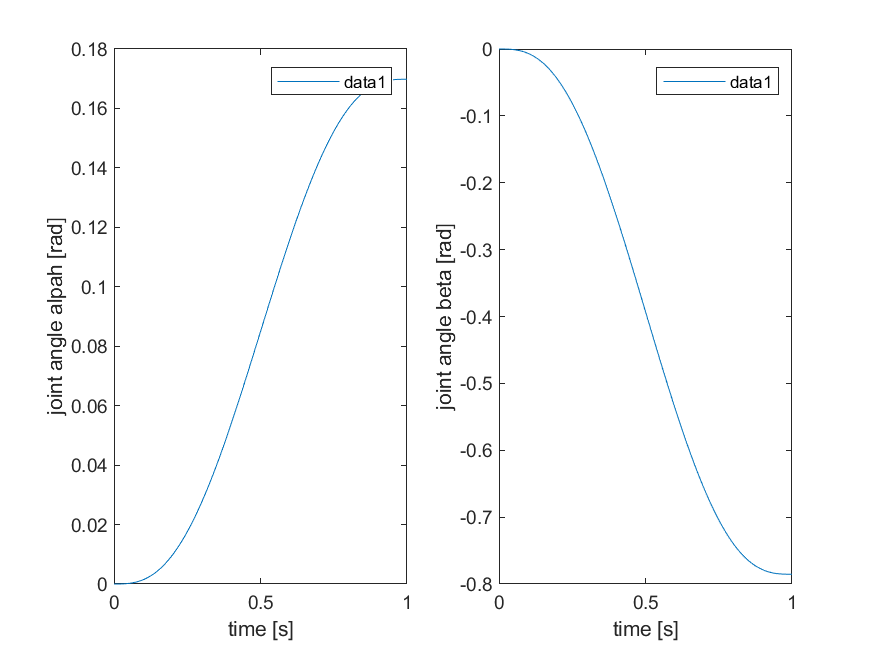
\includegraphics[width=0.95\textwidth]{Trajektorie.png}
	\caption{Trajektorie für \(\alpha\) und \(\beta\) }
\end{figure}


\subsection*{Aufgabe 4 - Bewegungsgleichung in Matlab}

Unsere Gruppe hat sich dafür entschieden die Bewegungsgleichung und ihre Lösung direkt in MatLab zu implementieren. Wie bereits in A2 erläutert wurde, haben wir die Symbolic Toolbox von Matlab benutzt, um die Bewegungsgleichung aufzustellen.

Unser Ziel ist es nun gewesen die aufgestellte Ordinary Differential Equations (ODE) mithilfe eines Solvers wie Euler-Vorwärts zu lösen. Dafür haben wir die Funktion \texttt{ode45} benutzt, welche die ODE numerisch löst. Die Funktion \texttt{ode45} benötigt als Eingabe die ODE, die Anfangsbedingungen und den Zeitbereich, in dem die ODE gelöst werden soll. Als Ausgabe liefert die Funktion die Lösung der ODE in Form von Vektoren für die Zeit und die Lösung der ODE. 

Wie vorgegeben haben wir als Optionen des Solvers \texttt{ode45} die \texttt{RelTol} auf $10^{-4}$ und \texttt{AbsTol} auf $10^{-7}$ gesetzt. Die \texttt{RelTol} gibt die relative Toleranz an, die die Lösung der ODE haben darf. Die \texttt{AbsTol} gibt die absolute Toleranz an, die die Lösung der ODE haben darf. Die Toleranzen sind wichtig, da die Lösung der ODE numerisch berechnet wird und somit nicht exakt ist. Die Toleranzen geben an, wie genau die Lösung der ODE sein muss. Außerdem haben wir eine maximale Schrittweite gesetzt mithilfe von \texttt{MaxStep} $=3\cdot 10^{-3}$. 

\subsubsection[short]{Aufstellen der rechten Seite}

Nun benötigen wir noch eine rechte Seite

\begin{lstlisting}[caption={Aufruf der Funktion \texttt{ode45}},label={lst:ode45}]
    % Syntax: y_0 = [alpha; alpha_dot; beta; beta_dot, err_alpha, err_beta]
    y_0 = [pi/2; 0.5; -pi/5; -0.1; 0; 0];
    tspan = [0, 1];
    opts = odeset('RelTol', 1e-4, ...
          'AbsTol', 1e-7, ...
          'MaxStep', 3*1e3);
    
    [t, y] = ode45(odefun, tspan, y0, opts);
\end{lstlisting}



\subsection*{Aufgabe 5 - Vorsteuerung und PID-Regler}

Um die Bewegungen des Roboters zur Endposition durchführen zu können, wurde eine Vorsteuerung und zwei PID-Regler entworfen.

Die Vorsteuerung nutzt die in Aufgabe 3 vordefinierten Trajektorien $(a_{\text{poly}}, b_{\text{poly}})$, um die erwarteten Gelenkwinkel q(t) als Vorgabe für das System bereitzustellen. Durch die Vorsteuerung wird die geplante Trajektorie aktiv in das Regelungssystem integriert. Gleichzeitig kompensiert der PID-Regler den entstehenden Fehler zwischen der geplanten Trajektorie und der tatsächlichen Gelenkposition aufgrund von Störungen im Reibterm.

Die Störungen im Reibterm führen zu falschen Drehmomenten an den Gelenken, was wiederum zu unerwünschten Beschleunigungen führt. Die Vorsteuerung agiert, indem sie die erwarteten Gelenkwinkel liefert und somit die gewünschte Fahrtrichtung vorgibt. Der PID-Regler wird dann verwendet, um aktiv auf Abweichungen zwischen der geplanten Trajektorie und der realen Bewegung des Systems zu reagieren.

Der Regelkreis ist somit in der Lage, die Auswirkungen der Störungen im Reibterm zu minimieren, indem er das Regelungssystem in Echtzeit anpasst. Die Vorsteuerung spielt dabei eine Schlüsselrolle bei der Vorgabe der idealen Bewegung, während der PID-Regler auf tatsächliche Abweichungen reagiert und diese korrigiert. Dieses koordinierte Zusammenspiel ermöglicht eine präzise und robuste Regelung, auch in Anwesenheit von Störungen, und stellt sicher, dass die geplante Trajektorie so genau wie möglich verfolgt wird.


Der Regler ist sowohl für \(\alpha\) als auch \(\beta\) implementiert. Die Eingangswerte umfassen die Lage, die Geschwindigkeit und den Regelabweichungsterm beider Gelenkwinkel. \(\text{Reg.Kp}\) ist der Proportionalgewichtungsfaktor, der die Stärke des proportionalen Regelterms steuert. Er beeinflusst die Regelabweichung \((x(1) - \text{reg.r\_alpha}(t))\), also die Abweichung der aktuellen Position unter der Trajektorie. \(\text{Reg.Ki}\) ist der Integralgewichtungsfaktor, der die Stärke des integralen Regelterms steuert. Dabei repräsentiert \(x(5)\) den kumulierten Fehler im Gelenkwinkel. \(\text{Reg.Kd}\) ist der Derivativgewichtungsfaktor, der die Stärke des derivativen Regelterms steuert. Dieser Term reagiert auf die Änderungsrate des Fehlers und glättet die Regelung.


\begin{verbatim}

assuming x -> [alpha; alpha_dot; beta; beta_dot; err_alpha; err_beta]
reg.pid = @(t, x) [-reg.Kp*(x(1)-reg.r_alpha(t))-reg.Ki*x(5)-reg.Kd*x(2);...
                   -reg.Kp*(x(3)- reg.r_beta(t))-reg.Ki*x(6)-reg.Kd*x(4)];
\end{verbatim}


Der gesamte Ausdruck gewährleistet eine präzise und stabile Verfolgung der vorgegebenen Sollwerte \( \text{reg.r\_alpha}(t) \) und \( \text{reg.r\_beta}(t) \) durch die Gelenke. Dabei tragen die verschiedenen Terme des PID-Reglers dazu bei, die Regelungseigenschaften anzupassen und auf unterschiedliche Aspekte des Regelproblems zu reagieren.

Für den PID-Regler werden folgende Werte verwendet:
\begin{verbatim}
    reg.Kp = 150;
    reg.Ki = 1;
    reg.Kd = 10;
\end{verbatim}
\subsection*{Aufgabe 6 - Störsignal}

Zur Modellierung eines Störsignals wird eine zufällige Zahl im Bereich von -1 bis 1 generiert. Diese Zufallszahl wird anschließend mit dem Faktor \( \text{reg.noise\_amp} = 5 \times 10^{-3} \) multipliziert. Dieser Vorgang wird für beide Reibungsterme unabhängig durchgeführt, da im realen Aufbau davon ausgegangen wird, dass sie nicht denselben Fehler aufweisen.

\[
\text{noise} = \text{reg.noise\_amp} \times 2 \times (\text{rand}(2,1) - 0.5)
\]

Dieser Ausdruck berechnet das Störsignal (\text{noise}) durch Multiplikation der zufälligen Zahlen im Bereich von -1 bis 1 mit dem angegebenen Faktor.


Das Störsignal wird nun auf die Stellgröße des Reglers \(u\) addiert, da es den gleichen Einfluss auf die Bewegungsgleichung wie der Reibterm \(Q\) hat.

\[ M(Q + u - D \cdot \dot{y}_{\text{punkt}} - G) \]

Die Stellgröße \(u\) wird durch die Addition des Störsignals korrigiert:

\[ u = u + \text{noise} \]

Der PID-Regler muss dieses Störsignal ausgleichen, da die tatsächlich gefahrene Strecke von der geplanten Trajektorie abweichen wird.


\subsection*{Resultat und Visualisierung}

Animiert wird die Bewegung des Knickarmroboters mithilfe des \texttt{plot} Befehls. Hierfür werden die bereits in Aufgabe 1 erläuterten homogenen Transformationsmatrizen genutzt, um die generalisierten Koordinaten $\alpha$ und $\beta$ auf kartesische Koordinaten zu übersetzen. Das erste Gelenk 

\begin{figure}[H]
    \centering
    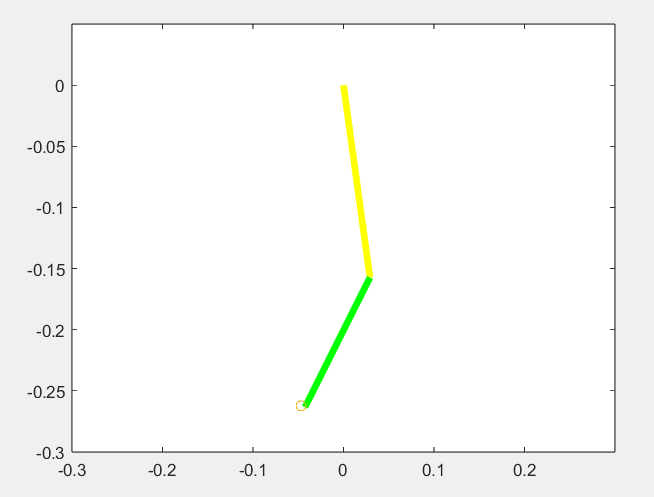
\includegraphics[width=0.8\linewidth]{img/visualisierung.png}
    \caption{Visualisierung der Simulation}
    \label{fig:visualisierung}
\end{figure}


\begin{lstlisting}[caption={Definition der rechten Seite},label={lst:wrapper}]
    %% Visualization
if plot_Ergebnis
    alphas = y(:, 1);
    betas = y(:, 3);
    [T_02, T_03] = dh_trafo();
    orig = [0 0 0 1]';
    time = [diff(t); 0];
    
    % Animation
    figure(1);
    % plots maximal 250 frames
    max_frame = 250;
    n_frame = min(size(y,1), max_frame);
    for frame=1:n_frame
        i = floor(frame/n_frame .* numel(t));
        G2 = T_02(alphas(i), betas(i))*orig;
        G3 = T_03(alphas(i), betas(i))*orig;
        plot_robot(G2, G3)
        hold on
        plot(y_end_glob(1), y_end_glob(2), "o")
        hold off
        drawnow;
        %wait such that the animation is as long as the simulated time
        pause(time(i));
    end
end
\end{lstlisting}




\subsection*{Diskussion}

\bibliographystyle{unsrt}
\bibliography{literature}

\end{document}